

\section{Problem 2}
\label{part2}
\begin{verbatim}

Choose a query term (e.g., ``shadow'') that is not a stop word
(see week 5 slides) and not HTML markup from step 1 (e.g., ``http'')
that matches at least 10 documents (hint: use ``grep'' on the processed
files).  If the term is present in more than 10 documents, choose
any 10 from your list.  (If you do not end up with a list of 10
URIs, you've done something wrong).

As per the example in the week 5 slides, compute TFIDF values for
the term in each of the 10 documents and create a table with the
TF, IDF, and TFIDF values, as well as the corresponding URIs.  The
URIs will be ranked in decreasing order by TFIDF values.  For
example:

Table 1. 10 Hits for the term ``shadow'', ranked by TFIDF.

TFIDF	TF	IDF	URI
-----	--	---	---
0.150	0.014	10.680	http://foo.com/
0.044	0.008	 5.510	http://bar.com/


You can use Google or Bing for the DF estimation.  To count the
number of words in the processed document (i.e., the deonminator
for TF), you can use ``wc'':

% wc -w www.cnn.com.processed
    2370 www.cnn.com.processed

It won't be completely accurate, but it will be probably be
consistently inaccurate across all files.  You can use more 
accurate methods if you'd like.  

Don't forget the log base 2 for IDF, and mind your significant
digits!

\end{verbatim}

\subsection{Solution}
\begin{enumerate}
\item Aim of this question is to first get 10 URIs which contains a specific key word in it. 
\item The keyword should not be a stop word like a,the,and etc and not html mark-up .I have chosen ``burger'' keyword.
\item So my first task was to write a program which takes 1000 URIs as input and gives all the list of URIs which have ``burger'' in it.
\item This can be done by using ``grep -lr'' command followed by ``burger''. This command is executed directly in putty in the folder which has all the 1000 processed files.
\item This gave me more than 10 files and that result is showed in Figure 6. I have randomly taken 10 URIs from this list and this list is shown in Figure 7.
\item Now in order to calculate TFIDF I need to calculate TF and IDF separately and then multiply both of them.
\item IDF is common for all the 10 URIs because it is based on the corpus. I have taken ``google'' as my search engine and I have found the total number of document in the corpus from reference 6. rel=mementos,rel=first memento and rel=memento last from the time maps..
\item Now I queried for ``burger'' in google which gave 263 million results which is the number of documents with burger in it. This is shown in Figure 5.
\item So my IDF will be total documents in corpus/263 million. This is same for all the 10 URIs.
\item IDF will be growing too large as corpus grows so in order to limit it I used log base 2 function of the IDF.  
\item Now TF can be calculated if we get the total number of words in each document and the number of occurrences of the word ``burger'' in each document.
\item I got the total number of words in each document using ``wc -w'' command followed by the file name of which I want the word count.
\item I got the number of times the word occurred in each document by using``grep -lr'' command followed by my keyword and followed by the file name in which the keyword should be searched.
\item By dividing occurrences/word count,I got TF. 
\item Now this TF is multiplied with IDF which gave me TFIDF value.
\item These TFIDF values for each URI are arranged in ascending order and these are shown in Figure 8.
\item The URI having high TFIDF value is first shown to the user when searched in a search engine.
  
\end{enumerate}
\newpage
\subsection{Code Listing}

\subsubsection{Python Code for getting URIs with ``burger'' and TFIDF values for each URI}
\lstinputlisting[language=Python,breaklines = true,frame=single,caption={Python Code for getting URIs with ``burger'' and TFIDF values for each URI}, label=lst:q1-1,captionpos=b,numbers=left,showspaces=false,showstringspaces=false,basicstyle=\footnotesize]{tfidf_final.py}
\newpage

\subsection{Results}

\subsubsection{Number of searches for ``burger'' in google}
\begin{figure}[ht]    
    \begin{center}
        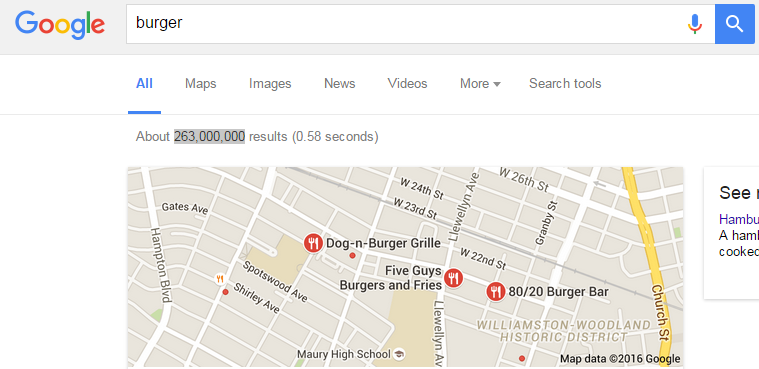
\includegraphics[scale=0.4]{burger_in_google.png}
        \caption{Number of searches for ``burger'' in google}
        \label{Number of searches for ``burger'' in google}
    \end{center}
\end{figure}

\subsubsection{Processed URI files- having ``burger'' keyword in it}
\begin{figure}[ht]    
    \begin{center}
        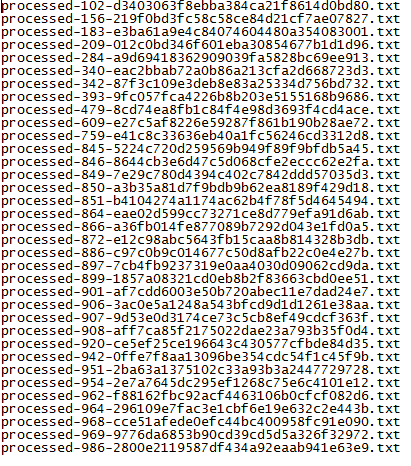
\includegraphics[scale=0.9]{uris_with_burger.png}
        \caption{Processed URI files- having ``burger'' keyword in it}
        \label{Processed URI files- having ``burger'' keyword in it}
    \end{center}
\end{figure}
\newpage
\subsubsection{10 random URIs from Processed URI files- having ``burger'' keyword in it}
\begin{figure}[ht]    
    \begin{center}
        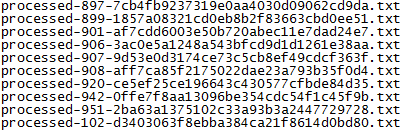
\includegraphics[scale=1]{10uris_with_burger.png}
        \caption{10 random URIs from Processed URI files- having ``burger'' keyword in it}
        \label{10 random URIs from Processed URI files- having ``burger'' keyword in it}
    \end{center}
\end{figure}

\subsubsection{TFIDF Table}
\begin{figure}[ht]    
    \begin{center}
        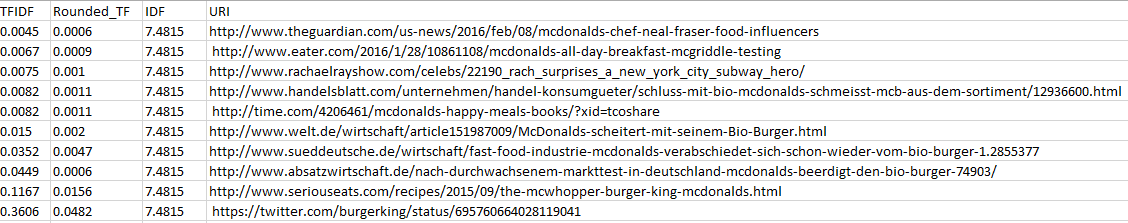
\includegraphics[scale=0.6]{Tfidf_table.png}
        \caption{TFIDF Table}
        \label{TFIDF Table}
    \end{center}
\end{figure}
\newpage
